\documentclass[a4paper,10pt]{article}
\usepackage[T1]{fontenc}
\usepackage[english]{babel}
\usepackage{mathtools}
\usepackage{bbm}
\usepackage{amsmath}
\usepackage{amsfonts}
\usepackage{amssymb}
\usepackage{fancyhdr}
\usepackage{geometry}
\usepackage{subfig}
\usepackage{enumerate}
\usepackage{graphicx}
\usepackage{caption}
\usepackage{subfig}
\usepackage{tabu}
\usepackage{multirow}
\usepackage{color}
\usepackage{listings}
\usepackage[]{algorithm2e}
\usepackage[autostyle,english=british]{csquotes}
\usepackage{minitoc}

\newtheorem{thm}{Theorem}
\newtheorem{defn}{Definition}
\newtheorem{prop}{Proposition}

%opening
\title{Technical Report about implementation in CUDA of Monte Carlo 
Linear Solvers (MCLS)}
\author{Steven Hamilton, Massimiliano Lupo Pasini}
\date{}

\begin{document}

\maketitle

\begin{abstract}
In this report timings are presented as concerns Monte 
Carlo Linear Solvers (MCLS) with different configurations. Different test 
cases are used to get quite a general overview of the behavior. 
In particular 
various options to generate random numbers as well as handling of data storage 
are 
tested for the sake of efficiency. All the test cases have been run three times 
to filter the fluctuations due to hardware issues. 
\end{abstract}

\section*{Introduction}
In this report different approaches are tested in order to maximize the 
performance of Monte Carlo linear solvers algorithms in GPU environment. 
Both Forward and Adjoint method are analyzed, pointing out the different 
implementation issues and pinpointing the different viable options to improve 
timings.
Four different numerical test cases are employed with different properties in 
terms of spectral radius of the iteration matrix, sparsity pattern, degrees 
of freedom and number of histories employed. The study is accomplished both by 
using a weight cutoff to kill the 
histories and by using a fixed number of steps for each of those, in order to 
discriminate the actual effectiveness of the different modifications 
introduced. An attempt to justify the improvements sometimes detected is 
provided, however a deeper understanding of the behaviors still has to be 
carried out. 



\section{Adjoint method - Different random number generation techniques}
The generation of random numbers plays an important role in the calculation of 
the solution to 
a linear system through a Monte Carlo procedure, since a new random number must 
be generated 
to either step ahead in a random walk or to kink off a new one.
Since this operation must be repeated very frequently in the code, it is 
recommendable to 
decrease its cost as much as possible, not to affect the efficiency of the 
overall performance.
Two viable options to initialize random number generators are:

\begin{enumerate}
 \item Having the same seed but different sequence number generates a number 
guaranteed 
to be $2^{67}$ away from each other, 
but the downside is the heavy computations to advance the $2^{67}$ position

\hspace*{-2cm}
\begin{lstlisting}
__global__ void initialize_rng(curandState *state, int seed, int offset)
{
    int tid = threadIdx.x + blockIdx.x * blockDim.x;

    curand_init(seed,tid,offset,&state[tid]);

}
\end{lstlisting}

\item Giving different seeds, and just keeping the sequence number at 0, 
it is a lot faster but there might be correlation between threads, since there 
is 
no 
guarantee on the separation between each threads. In this case the different 
seeds can be picked accordingly to different criteria. In this report we 
explore two approaches:
\begin{itemize}
 \item picking the seeds with consecutive indices
 \item picking the seeds with indices provided by a generator of integer random 
numbers
\end{itemize}

In case seeds with consecutive indices are chosen the set of instructions 
employed to generate the seed vector is the following:

\hspace*{-2cm}
\begin{lstlisting}
else if ( d_seed_type==SEED_TYPE::DIFF )
{
    std::cout<<"Different adjacent seeds instantiated"<<std::endl;

    thrust::device_vector<int> seeds( BLOCK_SIZE*num_blocks);
    thrust::sequence(seeds.begin(), seeds.end(), d_rng_seed);
    int* seed_ptr = thrust::raw_pointer_cast(seeds.data());

    initialize_rng<<<num_blocks, BLOCK_SIZE>>>(rng_states, seed_ptr,
        d_num_curand_calls, d_seed_type);
}

\end{lstlisting}

Instead in the case of seeds chosen with random indices the set of instructions 
executed is:

\hspace*{-2cm}
\begin{lstlisting}
else if ( d_seed_type==SEED_TYPE::RAND )
{
    std::cout<<"Different random seeds instantiated from 0 to "<<
    RAND_MAX<<std::endl;

    thrust::device_vector<int> dev_seeds( BLOCK_SIZE*num_blocks);
    thrust::host_vector<int> host_seeds( BLOCK_SIZE*num_blocks );
    std::srand(std::time(0));
    thrust::generate(host_seeds.begin(), host_seeds.end(), std::rand);
    dev_seeds=host_seeds;
    int* seed_ptr = thrust::raw_pointer_cast(dev_seeds.data());

    initialize_rng<<<num_blocks, BLOCK_SIZE>>>(rng_states, seed_ptr,
       d_num_curand_calls, d_seed_type);
}

\end{lstlisting}

The macro variable \texttt{RAND\_MAX} is set to 2147483647. Therefore 
we have the guarantee that a wide range of integers is spanned for the choice 
of the seeds.

In case as many seeds as the number of threads are 
employed, the kernel remains the same independently of the policy adopted for 
the selection of the seeds.

\hspace*{-2cm}
\begin{lstlisting}
__global__ void initialize_rng(curandState *state, int*seed, int offset)
{
    int tid = threadIdx.x + blockIdx.x * blockDim.x;

    curand_init(seed[tid], 0, offset, &state[tid]);
}
\end{lstlisting}
\end{enumerate}

\begin{table}[!h]
\hspace*{-2cm}
\begin{tabular}{|c|c|c|c|c|c|c|}
\hline
\textbf{Matrix} & \textbf{Size} &\textbf{Nb. Histories} & \textbf{\% time rng} 
& \textbf{\% time kernel} & tot. time (ms)& rel. residual norm\\
\hline
2D Laplacian& 900 & $10^7$ & 36.0 & 64.0 & 299,563 & 0.0931241 \\
\hline 
1D shifted Laplacian& $10^6$ & $10^4$ & 0.05 & 99.5 & 50,016 & 12.3509\\
\hline
1D shifted Laplacian& $10^6$ & $10^7$ & 18.3 & 81.7 & 640,563 & 0.391686 \\
\hline
$\text{SP}_1$ & 25,568 & $10^7$ & 18.0 & 82.0 & 349,096 & 0.450792 \\
\hline
\end{tabular}
\caption{Adjoint method - Timings using same seed and different sequences.} 
\label{tab1}
\end{table}



\begin{table}[!h]
\hspace*{-2.5cm}
\begin{tabular}{|c|c|c|c|c|c|c|c|}
\hline
\textbf{Matrix} & \textbf{Size} &\textbf{Nb. Hist.} & \textbf{\% time rng} 
& \textbf{\% time kernel} & tot. time (ms)& rel. res. norm & Rel. Timing\\
\hline
2D Laplacian& 900 & $10^7$ & 0.0 & 100.0 & 191,818 & 0.119588 & 0.64 \\
\hline 
1D shift Laplacian& $10^6$ & $10^4$ & 0.0 & 100.0 & 35,351 & 12.3914 & 0.707\\
\hline
1D shift Laplacian& $10^6$ & $10^7$ & 0.0 & 100.0 & 517,788 & 0.408134 & 
0.808\\
\hline
$\text{SP}_1$ & 25,568 & $10^7$ & 0.0 & 100.0 & 241,671 & 0.397887 & 0.692\\
\hline
\end{tabular}
\caption{Adjoint method - Timings using different consecutive seeds and same 
sequence.} 
\label{tab2}
\end{table}



\begin{table}[!h]
\hspace*{-2.5cm}
\begin{tabular}{|c|c|c|c|c|c|c|c|}
\hline
\textbf{Matrix} & \textbf{Size} &\textbf{Nb. Hist.} & \textbf{\% time rng} 
& \textbf{\% time kernel} & tot. time (ms)& rel. res. norm & Rel. Timing\\
\hline
2D Laplacian& 900 & $10^7$ & 0.0 & 100.0 & 193,381 & 0.112068 & 0.64\\
\hline 
1D shift Laplacian& $10^6$ & $10^4$ & 0.0 & 100.0 & 36,295 & 12.3404 & 0.726\\
\hline
1D shift Laplacian& $10^6$ & $10^7$ & 0.0 & 100.0 & 549,992 & 0.408296 & 
0.859\\
\hline
$\text{SP}_1$ & 25,568 & $10^7$ & 0.0 & 100.0 & 241,817 & 0.383815 & 0.693\\
\hline
\end{tabular}
\caption{Adjoint method - Timings using different seeds picked randomly and 
same 
sequence.} 
\label{tab3}
\end{table}



As it can be noticed from the previous Tables \ref{tab1}, \ref{tab2} and 
\ref{tab3}, the second and third options 
provides better timings. However the payoff 
is an increase of the final relative residual, likely due to the correlation 
between the sequences generated by different seeds.
The quantities "time rng" and "time kernel" are expressed in terms of percentage 
of the total time.

\section{Adjoint method - Use of texture memory}


The LDG instruction (exposed via the \texttt{\_\_ldg} intrinsic) is a memory 
load that uses the texture path. 
It has the advantage that it does not require the explicit use of textures, 
since it does not 
explicitly bind one. 
Therefore \texttt{\_\_ldg()} reads data through the texture path, without 
requiring a texture itself. 
It is an overloaded function with the prototype \texttt{\_\_ldg(const *T)} 
where T is one of CUDA's built-in types. 
The perk of using LDG instruction is that explicit uses of textures cause a 
certain 
amount of code clutter and overhead (e.g. for API calls to bind textures).
Classical textures also use the texture load path, but in addition can transform 
both index (e.g. clamping modes) 
and data returned (e.g. interpolation) in various ways; the necessary control 
information 
is provided to the hardware during texture binding.
Because the texture cache is non-coherent with 
respect to writes in the same kernel, use of the texture load path requires that 
the underlying data 
is read-only across the entire kernel.



\section{Adjoint method - LDG calls into the code}

LDG instructions have been introduced in the following functions of Profugus 
code:

\begin{enumerate}
 \item \texttt{lower\_bound}
 \item \texttt{initialize\_history}
 \item \texttt{getNewState}
 \item \texttt{tallyContribution}
\end{enumerate}


All the instructions employed above provide a runtime decrease. However, some of 
them are more
significant than others. In particular the most effective calls are the ones 
located in
1) and 3). This is due to the fact that these functions are the ones called most 
frequently.
The option of using LDG instruction at point 4) actually plays a role just when 
the expected value
estimator is employed.

In the examples represented below the length of the history is set to 10000 
steps. The simulations have been accomplished both with and without a weight 
cut off equal to $10^{-9}$.


\begin{table}[!h]
\begin{tabular}{|c|c|c|c|c|c|}
\hline
\textbf{Matrix} & \textbf{Size} &\textbf{Nb. Histories} & $\rho(H)$ 
& $\rho(\hat{H})$ & tot. time (ms)\\
\hline
2D Laplacian& 900 & $10^7$ & 0.994869 & 0.99447 & 191,818 \\
\hline 
1D shifted Laplacian& $10^6$ & $10^4$ & 0.799972 & 0.639977 & 35,351\\
\hline
1D shifted Laplacian& $10^6$ & $10^7$ & 0.799972 & 0.639977 & 517,788\\
\hline
$\text{SP}_1$ & 25,568 & $10^7$ & 0.977674 & 0.999836 & 241,671\\
\hline
\end{tabular}
\caption{Adjoint method - Timings without LDG instructions and constant history 
length equal to 
10,000.}
\label{tab4}
\end{table}


\begin{table}[!h]
\hspace*{-1cm}
\begin{tabular}{|c|c|c|c|c|c|c|}
\hline
\textbf{Matrix} & \textbf{Size} &\textbf{Nb. Histories} & $\rho(H)$ 
& $\rho(\hat{H})$ & tot. time (ms)& Rel. Timing\\
\hline
2D Laplacian& 900 & $10^7$ & 0.994869 & 0.99447 & 139,882 & 0.729\\
\hline 
1D shifted Laplacian& $10^6$ & $10^4$ & 0.799972 & 0.639977 & 37,610 & 1.064\\
\hline
1D shifted Laplacian& $10^6$ & $10^7$ & 0.799972 & 0.639977 & 500,092 & 0.966\\
\hline
$\text{SP}_1$ & 25,568 & $10^7$ & 0.977674 & 0.999836 & 157,545 & 0.652\\
\hline
\end{tabular}
\caption{Adjoint method - Timings with LDG instructions at 1) and constant 
history length equal 
to 
10,000.}
\label{tab5}
\end{table}


\begin{table}[!h]
\hspace*{-1cm}
\begin{tabular}{|c|c|c|c|c|c|c|}
\hline
\textbf{Matrix} & \textbf{Size} &\textbf{Nb. Histories} & $\rho(H)$ 
& $\rho(\hat{H})$ & tot. time (ms) & Rel. Timing\\
\hline
2D Laplacian& 900 & $10^7$ & 0.994869 & 0.99447 & 193,336 & 1.008\\
\hline 
1D shifted Laplacian& $10^6$ & $10^4$ & 0.799972 & 0.639977 & 37,759 & 1.068\\
\hline
1D shifted Laplacian& $10^6$ & $10^7$ & 0.799972 & 0.639977 & 548,909 & 1.060\\
\hline
$\text{SP}_1$ & 25,568 & $10^7$ & 0.977674 & 0.999836 & 241,490 & 1\\
\hline
\end{tabular}
\caption{Adjoint method - Timings with LDG instructions at 2) and constant 
history length equal 
to 
10,000.}
\label{tab6}
\end{table}


\begin{table}[!h]
\hspace*{-1cm}
\begin{tabular}{|c|c|c|c|c|c|c|}
\hline
\textbf{Matrix} & \textbf{Size} &\textbf{Nb. Histories} & $\rho(H)$ 
& $\rho(\hat{H})$ & tot. time (ms) & Rel. Timing\\
\hline
2D Laplacian& 900 & $10^7$ & 0.994869 & 0.99447 & 105,010 & 0.547\\
\hline 
1D shifted Laplacian& $10^6$ & $10^4$ & 0.799972 & 0.639977 & 36,340 & 1.028\\
\hline
1D shifted Laplacian& $10^6$ & $10^7$ & 0.799972 & 0.639977 & 519,408 & 1.003\\
\hline
$\text{SP}_1$ & 25,568 & $10^7$ & 0.977674 & 0.999836 & 200,559 & 0.830\\
\hline
\end{tabular}
\caption{Adjoint method - Timings with LDG instructions at 3) and constant 
history length equal 
to 
10,000.}
\label{tab7}
\end{table}


\begin{table}[!h]
\hspace*{-1cm}
\begin{tabular}{|c|c|c|c|c|c|c|}
\hline
\textbf{Matrix} & \textbf{Size} &\textbf{Nb. Histories} & $\rho(H)$ 
& $\rho(\hat{H})$ & tot. time (ms) & Rel. Timing\\
\hline
2D Laplacian& 900 & $10^7$ & 0.994869 & 0.99447 & 140,347 & 0.732\\
\hline 
1D shifted Laplacian& $10^6$ & $10^4$ & 0.799972 & 0.639977 & 36,344 & 1.028\\
\hline
1D shifted Laplacian& $10^6$ & $10^7$ & 0.799972 & 0.639977 & 499,007 & 0.964\\
\hline
$\text{SP}_1$ & 25,568 & $10^7$ & 0.977674 & 0.999836 & 157,458 & 0.652\\
\hline
\end{tabular}
\caption{Adjoint method - Timings with LDG instructions at 1), 2) and constant 
history length 
equal 
to 
10,000.}
\label{tab8}
\end{table}


\begin{table}[!h]
\hspace*{-1cm}
\begin{tabular}{|c|c|c|c|c|c|c|}
\hline
\textbf{Matrix} & \textbf{Size} &\textbf{Nb. Histories} & $\rho(H)$ 
& $\rho(\hat{H})$ & tot. time (ms)& Rel. Timing\\
\hline
2D Laplacian& 900 & $10^7$ & 0.994869 & 0.99447 & 105,166 & 0.548\\
\hline 
1D shifted Laplacian& $10^6$ & $10^4$ & 0.799972 & 0.639977 & 36,141 & 1.022\\
\hline
1D shifted Laplacian& $10^6$ & $10^7$ & 0.799972 & 0.639977 & 547,777 & 1.052\\
\hline
$\text{SP}_1$ & 25,568 & $10^7$ & 0.977674 & 0.999836 & 200,325 & 0.829\\
\hline
\end{tabular}
\caption{Adjoint method - Timings with LDG instructions at 2), 3) and constant 
history length 
equal 
to 
10,000.}
\label{tab9}
\end{table}


\begin{table}[!h]
\hspace*{-1cm}
\begin{tabular}{|c|c|c|c|c|c|c|}
\hline
\textbf{Matrix} & \textbf{Size} &\textbf{Nb. Histories} & $\rho(H)$ 
& $\rho(\hat{H})$ & tot. time (ms) & Rel. Timing\\
\hline
2D Laplacian& 900 & $10^7$ & 0.994869 & 0.99447 & 105,331 & 0.549\\
\hline 
1D shifted Laplacian& $10^6$ & $10^4$ & 0.799972 & 0.639977 & 34,616 & 0.979\\
\hline
1D shifted Laplacian& $10^6$ & $10^7$ & 0.799972 & 0.639977 & 520,762 & 1.006\\
\hline
$\text{SP}_1$ & 25,568 & $10^7$ & 0.977674 & 0.999836 & 138,091 & 0.571\\
\hline
\end{tabular}
\caption{Adjoint method - Timings with LDG instructions at 1), 2), 3) and 
constant history 
length 
equal 
to 
10,000.}
\label{tab10}
\end{table}



\begin{table}[!h]
\begin{tabular}{|c|c|c|c|c|c|c|}
\hline
\textbf{Matrix} & \textbf{Size} &\textbf{Nb. Histories} & $\rho(H)$ 
& $\rho(\hat{H})$ & tot. time (ms)\\
\hline
2D Laplacian& 900 & $10^7$ & 0.994869 & 0.99447 & 27,686\\
\hline 
1D shifted Laplacian& $10^6$ & $10^4$ & 0.799972 & 0.639977 & 35,108\\
\hline
1D shifted Laplacian& $10^6$ & $10^7$ & 0.799972 & 0.639977 & 40,720\\
\hline
$\text{SP}_1$ & 25,568 & $10^7$ & 0.977674 & 0.999836 & 4,919\\
\hline
\end{tabular}
\caption{Adjoint method - Timings without LDG instructions and with weight 
cutoff.}
\label{tab11}
\end{table}



\begin{table}[!h]
\hspace*{-1cm}
\begin{tabular}{|c|c|c|c|c|c|c|}
\hline
\textbf{Matrix} & \textbf{Size} &\textbf{Nb. Histories} & $\rho(H)$ 
& $\rho(\hat{H})$ & tot. time (ms) & Rel. Timing\\
\hline
2D Laplacian& 900 & $10^7$ & 0.994869 & 0.99447 & 26,344 & 0.952\\
\hline 
1D shifted Laplacian& $10^6$ & $10^4$ & 0.799972 & 0.639977 & 35,911 & 1.023\\
\hline
1D shifted Laplacian& $10^6$ & $10^7$ & 0.799972 & 0.639977 & 41,092 & 1.009\\
\hline
$\text{SP}_1$ & 25,568 & $10^7$ & 0.977674 & 0.999836 & 4,759 & 0.967\\
\hline
\end{tabular}
\caption{Adjoint method - Timings with LDG instructions at 1) and with weight 
cutoff.}
\label{tab12}
\end{table}



\begin{table}[!h]
\hspace*{-1cm}
\begin{tabular}{|c|c|c|c|c|c|c|}
\hline
\textbf{Matrix} & \textbf{Size} &\textbf{Nb. Histories} & $\rho(H)$ 
& $\rho(\hat{H})$ & tot. time (ms)& Rel. Timing\\
\hline
2D Laplacian& 900 & $10^7$ & 0.994869 & 0.99447 & 27,722 & 1.001\\
\hline 
1D shifted Laplacian& $10^6$ & $10^4$ & 0.799972 & 0.639977 & 36,005 & 1.026\\
\hline
1D shifted Laplacian& $10^6$ & $10^7$ & 0.799972 & 0.639977 & 40,001 & 0.982\\
\hline
$\text{SP}_1$ & 25,568 & $10^7$ & 0.977674 & 0.999836 & 5,585 & 1.135\\
\hline
\end{tabular}
\caption{Adjoint method - Timings with LDG instructions at 2) and with weight 
cutoff.}
\label{tab13}
\end{table}



\begin{table}[!h]
\hspace*{-1cm}
\begin{tabular}{|c|c|c|c|c|c|c|}
\hline
\textbf{Matrix} & \textbf{Size} &\textbf{Nb. Histories} & $\rho(H)$ 
& $\rho(\hat{H})$ & tot. time (ms) & Rel. Timing\\
\hline
2D Laplacian& 900 & $10^7$ & 0.994869 & 0.99447 & 24,814 & 0.896\\
\hline 
1D shifted Laplacian& $10^6$ & $10^4$ & 0.799972 & 0.639977 & 36,604 & 1.043\\
\hline
1D shifted Laplacian& $10^6$ & $10^7$ & 0.799972 & 0.639977 & 40,305 & 0.99\\
\hline
$\text{SP}_1$ & 25,568 & $10^7$ & 0.977674 & 0.999836 & 5,065 & 1.03\\
\hline
\end{tabular}
\caption{Adjoint method - Timings with LDG instructions at 3) and with weight 
cutoff.}
\label{tab14}
\end{table}


\begin{table}[!h]
\hspace*{-1cm}
\begin{tabular}{|c|c|c|c|c|c|c|}
\hline
\textbf{Matrix} & \textbf{Size} &\textbf{Nb. Histories} & $\rho(H)$ 
& $\rho(\hat{H})$ & tot. time (ms) & Rel. Timing\\
\hline
2D Laplacian& 900 & $10^7$ & 0.994869 & 0.99447 & 26,248 & 0.948\\
\hline 
1D shifted Laplacian& $10^6$ & $10^4$ & 0.799972 & 0.639977 & 35,741 & 1.018\\
\hline
1D shifted Laplacian& $10^6$ & $10^7$ & 0.799972 & 0.639977 & 40,017 & 0.983\\
\hline
$\text{SP}_1$ & 25,568 & $10^7$ & 0.977674 & 0.999836 & 4,701 & 0.956\\
\hline
\end{tabular}
\caption{Adjoint method - Timings with LDG instructions at 1) and 2) and with 
weight cutoff.}
\label{tab15}
\end{table}



\begin{table}[!h]
\hspace*{-1cm}
\begin{tabular}{|c|c|c|c|c|c|c|}
\hline
\textbf{Matrix} & \textbf{Size} &\textbf{Nb. Histories} & $\rho(H)$ 
& $\rho(\hat{H})$ & tot. time (ms) & Rel. Timing\\
\hline
2D Laplacian& 900 & $10^7$ & 0.994869 & 0.99447 & 27,184 & 0.982\\
\hline 
1D shifted Laplacian& $10^6$ & $10^4$ & 0.799972 & 0.639977 & 36,141 & 1.029\\
\hline
1D shifted Laplacian& $10^6$ & $10^7$ & 0.799972 & 0.639977 & 40,727 & 1\\
\hline
$\text{SP}_1$ & 25,568 & $10^7$ & 0.977674 & 0.999836 & 5,086 & 1.034\\
\hline
\end{tabular}
\caption{Adjoint method - Timings with LDG instructions at 2), 3) and with 
weight cutoff.}
\label{tab16}
\end{table}




\begin{table}[!h]
\hspace*{-1cm}
\begin{tabular}{|c|c|c|c|c|c|c|}
\hline
\textbf{Matrix} & \textbf{Size} &\textbf{Nb. Histories} & $\rho(H)$ 
& $\rho(\hat{H})$ & tot. time (ms)& Rel. Timing\\
\hline
2D Laplacian& 900 & $10^7$ & 0.994869 & 0.99447 & 24,307 & 0.878\\
\hline 
1D shifted Laplacian& $10^6$ & $10^4$ & 0.799972 & 0.639977 & 36,980 & 1.053\\
\hline
1D shifted Laplacian& $10^6$ & $10^7$ & 0.799972 & 0.639977 & 40,596 & 0.997\\
\hline
$\text{SP}_1$ & 25,568 & $10^7$ & 0.977674 & 0.999836 & 4,921 & 1\\
\hline
\end{tabular}
\caption{Adjoint method - Timings with LDG instructions at 1), 2) and 3) and 
with weight cutoff.}
\label{tab17}
\end{table}


In Tables \ref{tab5}-\ref{tab10} the relative timing is compared with the 
reference values in Table \ref{tab4}. Tables \ref{tab12}-\ref{tab17} contain 
relative timings with respect to the reference values in Table \ref{tab11}.


By comparing the values of Tables \ref{tab4}-\ref{tab11} it is pointed out that 
a benefit in terms of timings is achieved 
when \texttt{ldg} instructions are employed in all the three subroutines at 
issue.
Moreover the improvement is more 
evident for the 2D laplacian and the $SP_1$ matrix. The reason of this might be 
associated with the sparsity pattern. 
Indeed a higher number of nonzero entries induces the histories to run for 
longer, enhancing the utility of the 
texture memory might increase as well. For the 2D laplacian and the $SP_1$ 
matrix the employment of \texttt{\_\_ldg} 
instructions almost halves the time for the computation. 
In particular the instruction which seems to be more effective is the one 
located in the \texttt{getNewState} subroutine.
The time reduction gets 
weaker for the other test cases. In fact for the 1D laplacian it seems there is 
no benefit in terms of timings coming from the texture memory. 

By looking at the results of the same test cases when a weight cutoff is used, 
we can see that the utility of \texttt{\_\_ldg} instructions is almost vanished 
(see 
Tables \ref{tab12}-\ref{tab17}). It still plays a significant role for the 2D 
Laplacian, plausibly because of the spectral radius $\rho(H)\approx 1$ which 
induces the histories to run for many steps even when the cutoff is employed. 
For the other cases instead the spectral radius is so small that the weight 
cutoff kills the histories too son for the texture memory to be effective.

\section{Adjoint method - Generation of random numbers}

Random numbers must be employed for each random walk to:
\begin{itemize}
 \item determine what is the initial state
 \item determine the following state in the path accordingly to the current one
\end{itemize}


Essentially the generation of random numbers is located in the subroutines:
\begin{enumerate}
\item \texttt{initializeHistory}
\item \texttt{getNewState}
\end{enumerate}

These two operations have to be repeated for all the random walks employed in 
the computations. 
In order to minimize the time spent in the generation of random numbers, it 
might be useful
to gather the generation of many of these at the same time. 
Therefore a gathering of the random number generator's calls has been 
accomplished, partially modifying 
the subroutines "\texttt{initializeHistory}" and "\texttt{getNewState}".
The relationship one-to-one between the generation of a random number and a call 
to one of these two 
subroutines is broken. A group of random numbers is generated in advance before 
the call to the
aforementioned functions. The size of the batch for this grouped random numbers 
is a parameter that can be tuned to find the optimal configuration, 
reducing the total time 
of execution.

The viable options that might be adopted are:
\begin{enumerate}
 \item to call separately the random number generator once for the 
initializeHistory and then
   employ the batch for the successive steps
  \item to start employing the batch even for the initial step of the history 
\end{enumerate}



\begin{table}[!h]
\hspace*{-2.5cm}
\begin{tabular}{|c|c|c|c|c|c|c|c|}
\hline
\textbf{Matrix} & \textbf{Size} &\textbf{Nb. Hist} & \textbf{\% time rng} 
& \textbf{\% time kernel} & tot. time (ms)& rel. res. norm & Rel. Timing\\
\hline
2D Laplacian& 900 & $10^7$ & 0.0 & 100.0 & 192,325 & 0.119588 & 1.003\\
\hline 
1D shift Laplacian& $10^6$ & $10^4$ & 0.0 & 100.0 & 36,602 & 12.3914 & 1.035\\
\hline
1D shift Laplacian& $10^6$ & $10^7$ & 0.0 & 100.0 & 517,536 & 0.408134 & 1\\
\hline
$\text{SP}_1$ & 25,568 & $10^7$ & 0.0 & 100.0 & 241,928 & 0.397887 & 1.001\\
\hline
\end{tabular}
\caption{Adjoint method - Results for a single call of rng for both 
\texttt{initializeHistory} 
and \texttt{getNewState}.} 
\label{tab18}
\end{table}



\begin{table}[!h]
\hspace*{-2.5cm}
\begin{tabular}{|c|c|c|c|c|c|c|c|c|}
\hline
\textbf{Matrix} & \textbf{Size} &\textbf{Nb. Hist.} & \textbf{\% time rng} 
& \textbf{\% time kernel} & tot. time (ms)& rel. res. norm & Rel. Timing\\
\hline
2D Laplacian& 900 & $10^7$ & 0.0 & 100.0 & 22,634 & 0.119588 & 0.818\\
\hline 
1D shift Laplacian& $10^6$ & $10^4$ & 0.0 & 100.0 & 37,002 & 12.3914 & 1.054\\
\hline
1D shift Laplacian& $10^6$ & $10^7$ & 0.0 & 100.0 & 40,473 & 0.408134 & 0.994\\
\hline
$\text{SP}_1$ & 25,568 & $10^7$ & 0.0 & 100.0 & 4,806 & 0.397887 & 0.977\\
\hline
\end{tabular}
\caption{Adjoint method - Results for a single call of rng for both 
\texttt{initializeHistory} 
and \texttt{getNewState} with weight cut-off and use of ldg.} 
\label{tab19}
\end{table}

Overall, for a configuration where the length of the random walk is fixed, the 
two options seem to produce similar results (compare Tables \ref{tab4} 
and \ref{tab18}). Slightly better results are obtained instead with the second 
approach (compare values in Tables \ref{tab11} and \ref{tab19}) when a weight 
cutoff is used to terminate the histories. 

The time reduction accomplished by grouping the generation of several random 
numbers has not produced significant effects though. Therefore
from now on \texttt{initializeHistory} and \texttt{getNewState} will be 
employed by making an explicit call to the random number generator every time 
that is 
necessary to produce a new random number. 


\section{Adjoint method - Reorganization of data through \texttt{struct}}

In order to attempt the reduction of GPU timings, a 
reorganization of the matrices used by the Monte Carlo 
linear solver is accomplished.

In particular the pursue is to increase the vicinity of data that are going to 
be consulted in adjacent time steps by the computer.
Because of this a C++ \texttt{struct} has been introduced:
\hspace*{-2cm}
\begin{lstlisting}
struct device_row_data{
        double H;
        double P;
        double W;
        int inds;
};
\end{lstlisting}

When a new state 
has to be taken by a random walk, corresponding values of the 
transition probability, iteration matrix and weight are picked from the memory 
storage, providing the motivation for this attempt. The integer \texttt{inds} 
is used to store the index of the state, 
while the double values \texttt{H}, \texttt{P} and \texttt{W} are employed to 
store the entries of the iteration matrix, probability and weight respectively. 
This way, values of H, P, W associated with a particular entry are stored in 
contiguous cells of the memory.


This allows to reorganize the data necessary for the Monte Carlo linear solver 
in an array whose entries are \texttt{struct} elements. The length of the array 
corresponds to the number of nonzero entries of the iteration matrix.

In the following tables results associated with the employment of such data 
structure are presented, both by using a fixed length for the histories and by 
resorting to a weight cutoff of $10^{-9}$.


\begin{table}[!h]
\hspace*{-1cm}
\begin{tabular}{|c|c|c|c|c|c|c|}
\hline
\textbf{Matrix} & \textbf{Size} &\textbf{Nb. Histories} & $\rho(H)$ 
& $\rho(\hat{H})$ & tot. time (ms) & Rel. Timing\\
\hline
2D Laplacian& 900 & $10^7$ & 0.994869 & 0.99447 & 105,093 & 0.998\\
\hline 
1D shifted Laplacian& $10^6$ & $10^4$ & 0.799972 & 0.639977 & 27,404 & 0.792\\
\hline
1D shifted Laplacian& $10^6$ & $10^7$ & 0.799972 & 0.639977 & 422,197 & 0.811\\
\hline
$\text{SP}_1$ & 25,568 & $10^7$ & 0.977674 & 0.999836 & 138,921& 1.006\\
\hline
\end{tabular}
\caption{Adjoint method - Timings with \texttt{struct} data used and without 
weight cutoff. LDG 
instructions at 1), 2) and 
3)}
\label{tab20}
\end{table}



\begin{table}[!h]
\hspace*{-1cm}
\begin{tabular}{|c|c|c|c|c|c|c|}
\hline
\textbf{Matrix} & \textbf{Size} &\textbf{Nb. Histories} & $\rho(H)$ 
& $\rho(\hat{H})$ & tot. time (ms) & Rel. Timing\\
\hline
2D Laplacian& $900$ & $10^7$ & 0.994869 & 0.99447 & 24,669 & 1.015\\
\hline 
1D shifted Laplacian& $10^6$ & $10^4$ & 0.799972 & 0.639977 & 26,907 & 0.728\\
\hline
1D shifted Laplacian& $10^6$ & $10^7$ & 0.799972 & 0.639977 & 30,773 & 0.758\\
\hline
$\text{SP}_1$ & $25,568$ & $10^7$ & 0.977674 & 0.999836 & 5,005 & 1.017\\
\hline
\end{tabular}
\caption{Adjoint method - Timings with \texttt{struct} data used. LDG 
instructions at 1), 2) and 
3) and with weight cutoff.}
\label{tab21}
\end{table}


Looking at both results in Tables \ref{tab20} and \ref{tab21} it is pointed out 
that the reorganization of data does not introduce any benefits as regards the 
2D Laplacian or the $SP_1$ matrix. However significant reduction of timings are 
obtained for the 1D shifted Laplacian. 


\section{Forward method - Assignment of tasks to threads}


In the Adjoint method a single history contributes in the 
evaluation of different entries of the solution vector accordingly to the 
actual state visited. The Forward method instead is defined such that a single 
history always contributes on the same entry of the solution 
vector, depending on the state from which it has been initiated.


This typical property of the Forward method opens the way to different 
techniques to distribute the tasks between threads. In the problems at issue 
the concept of task coincide with a single history. Therefore the intent is to 
discover what is the best way to map histories to different threads accordingly 
to their index. 


Regardless of the amount o histories employed for a single entry (when this 
number is bigger than one), two viable options to execute the assignment are:

\begin{itemize}
 \item to employ different threads for the estimation of an entry of the 
solution vector
\item create a one-to-one relationship between the entries of the 
solution vector and the threads initialized during the process.
\end{itemize}

The first option induces to deal with the issue of different threads trying to 
modify the value of the same entry (data concurrency). From the 
point of view of implementation different approaches can be use to cope with 
it. In the following dissertation we proceed storing the solution 
vector in 
global memory and executing an atomization of all those operation that
access and modify values contained in the same memory cell.
The second approach, instead, does not entail any data concurrency since each 
thread always accesses a memory cell which is never consulted by any other 
thread. However we have a restriction to the number of threads which 
actually do a job, since it is necessarily  
equal to the size of the linear system.


The goal is to compare the timings between these two settings, focusing on 
determining the effects of the serialization occurring in the execution 
of the kernel for the first option.\newline

In the case when different threads are allowed to work on the same entry, a 
possible mapping might be the following one:

\hspace*{-2cm}
\begin{lstlisting}
__global__ void run_forward_monte_carlo(...)
{

    ...
   
    int tid = threadIdx.x + blockIdx.x * blockDim.x;
    int entry = tid / entry_histories;
    
    ...

}   
\end{lstlisting}

As already mentioned previously in the dissertation, this requires a 
serialization of the access by different threads to the same memory cell. This 
is accomplished by the following instruction:

\hspace*{-2cm}
\begin{lstlisting}
__device__ void tallyContribution(int state, double wt, double * const x)
{
        // Collision estimator just adds weight
        atomicAdd(x+state,wt);
}
\end{lstlisting}

The one-to-one relationship between entries and threads instead induces 
instead the following mapping:

\begin{lstlisting}
__global__ void run_forward_monte_carlo(...)
{

    ...
   
    int tid = threadIdx.x + blockIdx.x * blockDim.x;
    int entry = tid / entry_histories;
    
    ...

} 


\hspace*{-2cm}
\begin{lstlisting}
__global__ void run_forward_monte_carlo(...)
{

    ...
    
    int tid = threadIdx.x + blockIdx.x * blockDim.x; 
    if( tid < N )
    {
       ...
    }
    
    ...

}   
\end{lstlisting}


In the last case obviously it is necessary to instantiate a number of threads 
bigger than the actual size of the problem to solve, since in general the size 
of the blocks is not a divisor of the number of degrees of freedom. However, 
the higher is the size of the problem, the less this is an issue.\newline

For both the configurations the test cases are run both by using a fixed number 
of steps equal to 10,000 and by employing a weight cutoff equal to $10^{-9}$. 
No texture memory instructions are employed.


\begin{table}[!h]
\begin{tabular}{|c|c|c|c|c|c|}
\hline
\textbf{Matrix} & \textbf{Size} &\textbf{Nb. Histories per entry} & $\rho(H)$ 
& $\rho(\hat{H})$ & tot. time (ms)\\
\hline
2D Laplacian& $900$ & $10^3$ & 0.994869 & 0.99447 & 437,444 \\
\hline 
1D shifted Laplacian& $10^6$ & $5$ & 0.799972 & 0.639977 & 78,767\\
\hline
$\text{SP}_1$ & $25,568$ & $200$ & 0.977674 & 1.99619 & 241,573\\
\hline
\end{tabular}
\caption{Forward method - mapping of multiple threads to a single entry. Fixed 
number of steps equal to 10,000.}
\label{tab22}
\end{table}


\begin{table}[!h]
\hspace*{-1cm}
\begin{tabular}{|c|c|c|c|c|c|c|c|}
\hline
\textbf{Matrix} & \textbf{Size} &\textbf{Nb. Hist. per entry} & $\rho(H)$ 
& $\rho(\hat{H})$ & tot. time (ms) & Rel. Timing\\
\hline
2D Laplacian& $900$ & $10^3$ & 0.994869 & 0.99447 & 79,306 & 0.181\\
\hline 
1D shift Laplacian& $10^6$ & $5$ & 0.799972 & 0.639977 & 74,621 & 0.947\\
\hline
$\text{SP}_1$ & $25,568$ & $200$ & 0.977674 & 1.99619 & 122,773 & 0.508\\
\hline
\end{tabular}
\caption{Forward method - one-to-one mapping between threads and entries. Fixed 
number of steps equal to 10,000.}
\label{tab23}
\end{table}


Even if the case of the $SP_1$ matrix does not converge, we are going to 
consider the behavior of the code for this test case anyway. Indeed the 
priority is to
focus on the performance of the algorithm with respect to different 
instantiations of the threads rather than the accuracy of the final 
numerical result 
itself.

Comparing values in Tables \ref{tab22} and \ref{tab23}, we can see that the 
atomization of the contribution coming from each tally affect the 
performance of the algorithm for all the test cases analyzed, in particular for 
the 2D Laplacian and the $SP_1$ matrix. The outstanding improvement for these 
cases can be explained with the small size of the problems. 
In the first approach for the distribution of tasks, indeed, the tasks are 
attributed to the same entry according to a rotation of the blocks. Therefore 
threads working on the same entry of the solution vector will always belong to 
different blocks. In fact for a 
fixed block size, the higher is the size of the problem the lower is the 
contention of memory resources between threads belonging to different blocks.
This explains why results are pretty similar for the 1D shifted Laplacian, 
since its size is order of magnitudes bigger than for the other test cases 
analyzed.


\begin{table}[!h]
\hspace*{-1cm}
\begin{tabular}{|c|c|c|c|c|c|}
\hline
\textbf{Matrix} & \textbf{Size} &\textbf{Nb. Histories per entry} & $\rho(H)$ 
& $\rho(\hat{H})$ & tot. time (ms)\\
\hline
2D Laplacian& $900$ & $10^3$ & 0.994869 & 0.99447 & 206,439 \\
\hline 
1D shifted Laplacian& $10^6$ & $5$ & 0.799972 & 0.639977 & 39,295\\
\hline
$\text{SP}_1$ & $25,568$ & $200$ & 0.977674 & 1.99619 & 33,169\\
\hline
\end{tabular}
\caption{Forward method - mapping of multiple threads to a single entry. 
Weight cutoff equal to $10^{-9}$.}
\label{tab24}
\end{table}


\begin{table}[!h]
\hspace*{-1cm}
\begin{tabular}{|c|c|c|c|c|c|c|}
\hline
\textbf{Matrix} & \textbf{Size} &\textbf{Nb. Hist. per entry} & $\rho(H)$ 
& $\rho(\hat{H})$ & tot. time (ms) & Rel. Timing\\
\hline
2D Laplacian& $900$ & $10^3$ & 0.994869 & 0.99447 & 11,572 & 0.056\\
\hline 
1D shift Laplacian& $10^6$ & $5$ & 0.799972 & 0.639977 & 38,484 & 0.976\\
\hline
$\text{SP}_1$ & $25,568$ & $200$ & 0.977674 & 1.99619 & 6,505 & 0.196\\
\hline
\end{tabular}
\caption{Forward method - one-to-one mapping between threads and entries. 
Weight cutoff equal to $10^{-9}$.}
\label{tab25}
\end{table}

Looking at Tables \ref{tab24} and \ref{tab25}, the employment of 
the one-to-one map still has a huge impact in terms of performance as concerns 
that 2D Laplacian and the $SP_1$ matrix. As regards the 1D shifted Laplacian, 
instead, the weight cutoff seems to have e dominant effect on the timing, 
eliding the utility of the different techniques for the assignment of the tasks 
to the threads instantiated. A plausible explanation for this phenomenon might 
be 
the sparsity pattern of the matrices analyzed. In fact the number of nonzero 
entries per row is much higher for the first and third problem than for the 
second. Moreover the spectral radii of $H$ and $\hat{H}$ are much smaller for 
the shifted 1D Laplacian. Therefore the average 
number of steps per history is lower for the 1D shifted Laplacian than for the 
other cases, explaining why this particular problem is transparent to the 
employment of different mappings for the task distribution.


\section{Forward method - Use of texture memory}
We now focus on comparing the change of performance of the Forward method 
depending on whether texture memory instructions are used or not. 
The collocation of the texture memory instructions is the same as for the 
Adjoint method.

By default the one-to-one 
mapping for the execution of the tasks by different threads is employed. 
Results 
are shown both by resorting to a fixed length of the histories and also by 
using an adaptive weight cutoff.


\begin{table}[!h]
\hspace*{-1cm}
\begin{tabular}{|c|c|c|c|c|c|c|}
\hline
\textbf{Matrix} & \textbf{Size} &\textbf{Nb. Hist. per entry} & $\rho(H)$ 
& $\rho(\hat{H})$ & tot. time (ms)& Rel. Timing\\
\hline
2D Laplacian& $900$ & $10^3$ & 0.994869 & 0.99447 & 52,077 & 0.657\\
\hline 
1D shift Laplacian& $10^6$ & $5$ & 0.799972 & 0.639977 & 63,353 & 0.849\\
\hline
$\text{SP}_1$ & $25,568$ & $200$ & 0.977674 & 1.99619 & 72,198 & 0.588\\
\hline
\end{tabular}
\caption{Forward method - one-to-one mapping between threads and entries. Fixed 
number of steps equal to 10,000. LDG instructions employed.}
\label{tab26}
\end{table}

Comparing results in Table \ref{tab26} with the ones in Table \ref{tab23}, it 
is detected a significant improvement of the timings thanks to the employment 
of texture memory. Especially for the $SP_1$ matrix, supposedly for its 
sparsity pattern.


\begin{table}[!h]
\hspace*{-1cm}
\begin{tabular}{|c|c|c|c|c|c|c|}
\hline
\textbf{Matrix} & \textbf{Size} &\textbf{Nb. Hist. per entry} & $\rho(H)$ 
& $\rho(\hat{H})$ & tot. time (ms) & Rel. Timings\\
\hline
2D Laplacian& $900$ & $10^3$ & 0.994869 & 0.99447 & 9,316 & 0.805\\
\hline 
1D shift Laplacian& $10^6$ & $5$ & 0.799972 & 0.639977 & 40,005 & 1.04\\
\hline
$\text{SP}_1$ & $25,568$ & $200$ & 0.977674 & 1.99619 & 4,269 & 0.656\\
\hline
\end{tabular}
\caption{Forward method - one-to-one mapping between threads and entries. 
Weight cutoff equal to $10^{-9}$. LDG instructions employed.}
\label{tab27}
\end{table}

By making a comparison between Tables \ref{tab27} and \ref{tab25} we discover a 
similar behavior to the one verified for the Adjoint method. In fact once the 
weight cutoff is employed, the use of \texttt{\_\_ldg} instructions seem not to 
be effective for the reduction of the computational time.


\section{Forward method - Reorganization of data through \texttt{struct}}
In this section we focus on testing the efficiency of the employment of C++ 
\texttt{struct} objects to handle data, on the same lead as for the Adjoint 
method.
The experiments are repeated both for a fixed length of histories equal to 
10,000 and for the use of a weight cutoff equal to $10^{-9}$, with and without 
\texttt{ldg} instructions as well. The one-to-one mapping between 
tasks and threads is employed.


\begin{table}[!h]
\hspace*{-1cm}
\begin{tabular}{|c|c|c|c|c|c|c|}
\hline
\textbf{Matrix} & \textbf{Size} &\textbf{Nb. Hist per entry} & $\rho(H)$ 
& $\rho(\hat{H})$ & tot. time (ms) & Rel. Timing\\
\hline
2D Laplacian& $900$ & $10^3$ & 0.994869 & 0.99447 & 80,059 & 1.009\\
\hline 
1D shift Laplacian& $10^6$ & $5$ & 0.799972 & 0.639977 & 79,807 & 1.069\\
\hline
$\text{SP}_1$ & $25,568$ & $200$ & 0.977674 & 1.99619 & 122,861 & 1\\
\hline
\end{tabular}
\caption{Forward method - use of struct for data handling. One-to-one mapping 
between threads and entries. 
Fixed number of steps equal to 10,000. No LDG instructions.}
\label{tab28}
\end{table}


\begin{table}[!h]
\hspace*{-1cm}
\begin{tabular}{|c|c|c|c|c|c|c|}
\hline
\textbf{Matrix} & \textbf{Size} &\textbf{Nb. Hist. per entry} & $\rho(H)$ 
& $\rho(\hat{H})$ & tot. time (ms) & Rel. Timing\\
\hline
2D Laplacian& $900$ & $10^3$ & 0.994869 & 0.99447 & 11,534 & 1.003\\
\hline 
1D shift Laplacian& $10^6$ & $5$ & 0.799972 & 0.639977 & 29,636 & 0.770\\
\hline
$\text{SP}_1$ & $25,568$ & $200$ & 0.977674 & 1.99619 & 6,247 & 0.960\\
\hline
\end{tabular}
\caption{Forward method - use of struct for data handling. One-to-one mapping 
between threads and entries. 
Weight cutoff equal to $10^{-9}$. No LDG instructions.}
\label{tab29}
\end{table}



\begin{table}[!h]
\hspace*{-1cm}
\begin{tabular}{|c|c|c|c|c|c|c|}
\hline
\textbf{Matrix} & \textbf{Size} &\textbf{Nb. Hist. per entry} & $\rho(H)$ 
& $\rho(\hat{H})$ & tot. time (ms) & Rel. Timing\\
\hline
2D Laplacian& $900$ & $10^3$ & 0.994869 & 0.99447 & 50,159 & 0.627\\
\hline 
1D shift Laplacian& $10^6$ & $5$ & 0.799972 & 0.639977 & 67,993 & 0.852\\
\hline
$\text{SP}_1$ & $25,568$ & $200$ & 0.977674 & 1.99619 & 75,305 & 0.598\\
\hline
\end{tabular}
\caption{Forward method - use of struct for data handling. One-to-one mapping 
between threads and entries. 
Fixed number of steps equal to 10,000. LDG instructions employed.}
\label{tab30}
\end{table}


\begin{table}[!h]
\hspace*{-1cm}
\begin{tabular}{|c|c|c|c|c|c|c|}
\hline
\textbf{Matrix} & \textbf{Size} &\textbf{Nb. Hist. per entry} & $\rho(H)$ 
& $\rho(\hat{H})$ & tot. time (ms) & Rel. Timing\\
\hline
2D Laplacian& $900$ & $10^3$ & 0.994869 & 0.99447 & 8,950 & 1.041\\
\hline 
1D shift Laplacian& $10^6$ & $5$ & 0.799972 & 0.639977 & 30,314 & 0.758\\
\hline
$\text{SP}_1$ & $25,568$ & $200$ & 0.977674 & 1.99619 & 4,040 & 0.946\\
\hline
\end{tabular}
\caption{Forward method - use of struct for data handling. One-to-one mapping 
between threads and entries. 
Weight cutoff equal to $10^{-9}$. LDG instructions employed.}
\label{tab31}
\end{table}

Results in Tables \ref{tab28} (compared with Table \ref{tab23}) and \ref{tab29} 
show (compared with Table \ref{tab25}) show
that actually the employment of \texttt{struct} for the data storage does not 
provide 
improvements without using texture memory. However an 
interesting progress is detected for all the test cases at hand when use of 
\texttt{struct} and texture memory are combined for a fixed length of the 
histories. Moreover, on the same lead as for the Adjoin method, the 
effectiveness of all the modifications shades with a weight cutoff to shut down 
the random walks adaptively (compare results in Tables \ref{tab31} with the 
ones in Table \ref{tab27}).


\section{Use of L1 global cache}
Primary versions of NVIDIA graphic board were already garnered with L1 local 
cache memories. However they were not endowed with a similar memory to cache 
accesses to global memory which are known to cause the highest latency timings.
Using a caching system for such accesses can provide evident advantages, 
relatively to the particular application at hand and t its implementation. 


Recent versions of NVIDIA GPUs enable the use of L1 cache memories.
Tesla K40m graphic boards, the ones installed in Titan, belong to this set of 
processors. 

Even on Kepler GPUs that do support caching global memory in L1, the default 
behavior is to not cache global memory in L1. You have to opt-in to enable 
caching by passing \texttt{-Xptxas=-dlcm=ca} as an argument to NVCC when 
compiling your kernels. Kernels compiled in this fashion will still function on 
earlier Kepler devices though global memory operations will bypass the L1 cache.


You can programmatically query whether a GPU supports caching global 
memory operations using \texttt{cudaGetDeviceProperties} and examining the 
\texttt{globalL1CacheSupported} property.


In our code we have included the following commands in the main file in order 
to display the technical properties of GPUs at hand:

\hspace*{-2cm}
\begin{lstlisting}
  int nDevices;

  cudaGetDeviceCount(&nDevices);
  printf("The number of GPU devices is: %d\n", nDevices);
  for (int i = 0; i < nDevices; i++) {
    cudaDeviceProp prop;
    cudaGetDeviceProperties(&prop, i);
    printf("Device Number: %d\n", i);
    printf("  Device name: %s\n", prop.name);
    printf("  Memory Clock Rate (KHz): %d\n",
           prop.memoryClockRate);
    printf("  Memory Bus Width (bits): %d\n",
           prop.memoryBusWidth);
    printf("  Peak Memory Bandwidth (GB/s): %f\n\n",
           2.0*prop.memoryClockRate*(prop.memoryBusWidth/8)/1.0e6);
    printf("  globalL1CacheSupported:  %d\n", prop.globalL1CacheSupported);
    printf("  localL1CacheSupported:  %d\n", prop.localL1CacheSupported);
  }
\end{lstlisting}

One we have verified the presence of L1 Global caches in the NVDIA GPUs 
available, we can still customize even more the use for the resources at hand. 
In fact the L1 cache and the shared memory use a single memory for 
their purposes, splitting a common physical resources in two equal parts. In 
the case when either the shared memory or the L1 global cache are not used, it 
is pointless to keep occupied a part of memory for something tat will never be 
employed. Therefore it is possible to recalibrate the amount of Kbytes 
dedicated to both the kind of memories. 
This is possible through the use of two functions named 
\texttt{cudaDeviceSetCacheConfig} and \texttt{cudaFuncSetCacheConfig}. Their 
definition is included in the \texttt{cuda\_runtime\_api.h} header file.

The subroutine \texttt{cudaDeviceSetCacheConfig} requires only an argument, 
since its action affect the way all the subsequent kernels are executed. 
Instead \texttt{cudaFuncSetCacheConfig} requires two arguments. The first one 
is the name of the kernel to which it has to be applied, since it changes the 
handling of hardware resources between L1 cache and shared memory just for the 
specific kernel declared. 
The argument of \texttt{cudaDeviceSetCacheConfig} and the second one of 
\texttt{cudaFuncSetCacheConfig} can attain one of the following values:

\begin{itemize}
 \item \texttt{cudaFuncCachePreferShared}
 \item \texttt{cudaFuncCachePreferL1}
 \item \texttt{cudaFuncCachePreferEqual}
\end{itemize}

The third one corresponds to the default setting. The first one dedicate more 
memory cells to the shared memory, the second one instead shifts mos of it to 
the L1 cache use.\newline

It is possible to monitor the amount of resources used at runtime by passing 
some parameter to the NVIDIA profiler (NVPROF or NVVP). 
In the case of \texttt{nvprof} the command line looks like the one presented 
below here:
\hspace*{-2cm}
\begin{lstlisting}
 nvprof --metrics <type_of_counter> <executable_name> 
<arguments_for_executable>
\end{lstlisting}

The kind of counters that can be used as metric tools are:
\begin{itemize}
 \item \texttt{l1\_cache\_global\_hit\_rate} - percentage of reads that hit in 
L1 (Opt-In, K40/K80 only)
\item \texttt{tex\_cache\_hit\_rate} - percentage of reads that hit in texture 
cache (\_\_ldg() or texture access only) 
\item \texttt{l2\_l1\_read\_hit\_rate} - percentage of l1 misses which hit in L2
\item \texttt{l2\_texture\_read\_hit\_rate} - percentage of texture misses 
which hit in L2
\end{itemize}


All these counters provide you information regarding the use of hardware 
resources for each separate kernel employed in the code. 

For our current interest we use \texttt{l1\_cache\_global\_hit\_rate}. In the 
following treatise we present timings for the most important setting described 
before (for Adjoint and Forward MC), enabling the use of L1 global cache. 
Percentage of such resource used by the kernels are provided too. However, 
since 
the profiling affect the performance of the code, each configuration has been 
run twice for the sake of validity of the results presented: once without and 
once with the profiler. \newline

As regards the Adjoint method, enabling L1 global cache does not provide 
evident improvements, as it can be verified with results in Tables 
\ref{tab32}-\ref{tab37}. Sporadic time reductions occur for all the test cases 
considered but it is hard to find a correlation between the role played by the 
global cache memory and the other factors of the setting. In particular it is 
not possible to declare that such reductions are due to the global cache, since 
in most of the cases the profiler prompts out that no cache resources 
are actually employed. 


\begin{table}[!h]
\begin{tabular}{|c|c|c|c|c|c|}
\hline
\textbf{Matrix} & \textbf{Size} &\textbf{Nb. Hist.} & tot. time (ms)& \% rng - 
\% mc & Rel. Timing\\
\hline
2D Laplacian& 900 & $10^7$ & 167,270 & 0 - 0 & 0.874 \\
\hline 
1D shift Laplacian& $10^6$ & $10^4$ &  36,854 & 0 - 0 & 1.021\\
\hline
1D shift Laplacian& $10^6$ & $10^7$ & 573,288 & 0 - 0 & 1.075\\
\hline
$\text{SP}_1$ & 25,568 & $10^7$ & 306,248 & 0 - 0 & 1.268\\
\hline
\end{tabular}
\caption{Adjoint method - Use of L1 global cache. Fixed number of steps equal 
to 10,000. No LDG instructions. Relative Timings compared with Table 
\ref{tab4}.} 
\label{tab32}
\end{table}


\begin{table}[!h]
\begin{tabular}{|c|c|c|c|c|c|}
\hline
\textbf{Matrix} & \textbf{Size} &\textbf{Nb. Hist.} & tot. time (ms)& \% rng - 
\% mc & Rel. Timing\\
\hline
2D Laplacian& 900 & $10^7$ & 32,460 & 0 - 0 & 1.172 \\
\hline 
1D shift Laplacian& $10^6$ & $10^4$ &  38,002 & 0 - 0 & 1.082\\
\hline
1D shift Laplacian& $10^6$ & $10^7$ & 40,910 & 0 - 0 & 1.005\\
\hline
$\text{SP}_1$ & 25,568 & $10^7$ & 6,781 & 0 - 0 & 1.379\\
\hline
\end{tabular}
\caption{Adjoint method - Use of L1 global cache. Weight cutoff equal to 
$10^{-9}$. No LDG instructions. Relative Timings compared with Table 
\ref{tab11}.} 
\label{tab33}
\end{table}


\begin{table}[!h]
\begin{tabular}{|c|c|c|c|c|c|}
\hline
\textbf{Matrix} & \textbf{Size} &\textbf{Nb. Hist.} & tot. time (ms)& \% rng - 
\% mc & Rel. Timing\\
\hline
2D Laplacian& 900 & $10^7$ & 101,068 & 0 - 0 & 0.960 \\
\hline 
1D shift Laplacian& $10^6$ & $10^4$ &  36,776 & 0 - 0 & 1.062\\
\hline
1D shift Laplacian& $10^6$ & $10^7$ & 574,863 & 0 - 0 & 1.104\\
\hline
$\text{SP}_1$ & 25,568 & $10^7$ & 118,604 & 0 - 0 & 0.859\\
\hline
\end{tabular}
\caption{Adjoint method - Use of L1 global cache. Fixed number of steps equal 
to 10,000. LDG instructions employed. Relative Timings compared with Table 
\ref{tab10}.} 
\label{tab34}
\end{table}


\begin{table}[!h]
\begin{tabular}{|c|c|c|c|c|c|}
\hline
\textbf{Matrix} & \textbf{Size} &\textbf{Nb. Hist.} & tot. time (ms)& \% rng - 
\% mc & Rel. Timing\\
\hline
2D Laplacian& 900 & $10^7$ & 28,222 & 0 - 0 & 1.161 \\
\hline 
1D shift Laplacian& $10^6$ & $10^4$ &  36,042 & 0 - 0 & 0.975\\
\hline
1D shift Laplacian& $10^6$ & $10^7$ & 41,473 & 0 - 0 & 1.022\\
\hline
$\text{SP}_1$ & 25,568 & $10^7$ & 4,644 & 0 - 0 & 0.944\\
\hline
\end{tabular}
\caption{Adjoint method - Use of L1 global cache. Weight cutoff equal to 
$10^{-9}$. LDG instructions employed. Relative Timings compared with Table 
\ref{tab17}.} 
\label{tab35}
\end{table}


\begin{table}[!h]
\begin{tabular}{|c|c|c|c|c|c|}
\hline
\textbf{Matrix} & \textbf{Size} &\textbf{Nb. Hist.} & tot. time (ms)& \% rng - 
\% mc & Rel. Timing\\
\hline
2D Laplacian& 900 & $10^7$ & 101,004 & 0 - 0 & 0.961 \\
\hline 
1D shift Laplacian& $10^6$ & $10^4$ &  27,351 & 0 - 21.37 & 0.998\\
\hline
1D shift Laplacian& $10^6$ & $10^7$ & 413,696 & 0 - 0 & 0.980\\
\hline
$\text{SP}_1$ & 25,568 & $10^7$ & 133,346 & 0 - 0 & 0.96\\
\hline
\end{tabular}
\caption{Adjoint method - Use of \texttt{struct} for data handling. Use of L1 
global cache. Fixed number of steps equal 
to 10,000. LDG instructions employed. Relative Timings compared with Table 
\ref{tab20}.} 
\label{tab36}
\end{table}


\begin{table}[!h]
\begin{tabular}{|c|c|c|c|c|c|}
\hline
\textbf{Matrix} & \textbf{Size} &\textbf{Nb. Hist.} & tot. time (ms)& \% rng - 
\% mc & Rel. Timing\\
\hline
2D Laplacian& 900 & $10^7$ & 28,986 & 0 - 74.29 & 1.175 \\
\hline 
1D shift Laplacian& $10^6$ & $10^4$ &  26,838 & 0 - 0 & 0.997\\
\hline
1D shift Laplacian& $10^6$ & $10^7$ & 30,671 & 0 - 0 & 0.997\\
\hline
$\text{SP}_1$ & 25,568 & $10^7$ & 4,886 & 0 - 0 & 0.976\\
\hline
\end{tabular}
\caption{Adjoint method - Use of \texttt{struct} for data handling. Use 
of L1 global cache. Weight 
cutoff equal to $10^{-9}$. Relative Timings compared with Table 
\ref{tab21}.} 
\label{tab37}
\end{table}


Better results are obtained by activating L1 cache for the Forward method. In 
particular the combination of the use of \texttt{struct} and L1 global cache 
provides significant improvement of timings and cache resources are employed 
almost to the full for all the test cases considered. This phenomenon can be 
explained with the fact that the \texttt{struct} enables to reorder data so 
that values accessed in consecutive moments in time are physically close in the 
memory storage. Therefore caching information before using them helps in 
reducing the runtime effectively. 

A possible explanation for such discrepancy between 
Adjoint and Forward method is associated with the policy to estimate single 
entries of the solution vector. In fact the Forward method is characterized by 
a one-to-one relationship between the row of the iteration matrix and 
the entry for which such row provides contributions. It entails that in the 
Forward method consecutive states of the same random walk visit entries that 
are likely close in the compressed storage of the matrix. 

The same thing does not necessarily apply for the Adjoint method, since from 
one state to the consecutive one the row visited by the algorithm changes as 
well. Therefore, it is very likely that consecutive steps visit entries far one 
from the other in the matrix storage. L1 cache hardly provides benefits for 
time reduction in situations like these.

\begin{table}[!h]
\hspace*{-1cm}
\begin{tabular}{|c|c|c|c|c|c|}
\hline
\textbf{Matrix} & \textbf{Size} &\textbf{Nb. Hist. per entry} & tot. time 
(ms) & \% rng - 
\% mc  & Rel. Timing\\
\hline
2D Laplacian& $900$ & $10^3$ & 74,274 & 0 - 0 & 0.937\\
\hline 
1D shift Laplacian& $10^6$ & $5$ & 82,440 & 0 - 0 & 1.105\\
\hline
$\text{SP}_1$ & $25,568$ & $200$ & 197,493 & 0 - 0 & 1.609\\
\hline
\end{tabular}
\caption{Forward method. Fixed number of steps equal to 10,000. No LDG 
instructions. Relative Timings compared with Table 
\ref{tab23}.}
\label{tab38}
\end{table}



\begin{table}[!h]
\hspace*{-1cm}
\begin{tabular}{|c|c|c|c|c|c|}
\hline
\textbf{Matrix} & \textbf{Size} &\textbf{Nb. Hist. per entry} & tot. time 
(ms) & \% rng - 
\% mc  & Rel. Timing\\
\hline
2D Laplacian& $900$ & $10^3$ & 9,716 & 0 - 0 & 0.840\\
\hline 
1D shift Laplacian& $10^6$ & $5$ & 36,040 & 0 - 0 & 0.936\\
\hline
$\text{SP}_1$ & $25,568$ & $200$ & 8,189 & 0 - 0 & 1.259\\
\hline
\end{tabular}
\caption{Forward method. Weight cutoff equal to $10^{-9}$. No LDG 
instructions. Relative Timings compared with Table 
\ref{tab25}.}
\label{tab39}
\end{table}


\begin{table}[!h]
\hspace*{-1cm}
\begin{tabular}{|c|c|c|c|c|c|}
\hline
\textbf{Matrix} & \textbf{Size} &\textbf{Nb. Hist. per entry} & tot. time 
(ms) & \% rng - 
\% mc  & Rel. Timing\\
\hline
2D Laplacian& $900$ & $10^3$ & 44,134 & 0 - 0 & 0.847\\
\hline 
1D shift Laplacian& $10^6$ & $5$ & 52,816 & 0 - 0 & 0.834\\
\hline
$\text{SP}_1$ & $25,568$ & $200$ & 74,393 & 0 - 0 & 1.030\\
\hline
\end{tabular}
\caption{Forward method. Fixed number of steps equal to 10,000. LDG 
instructions employed. Relative Timings compared with Table 
\ref{tab26}.}
\label{tab40}
\end{table}



\begin{table}[!h]
\hspace*{-1cm}
\begin{tabular}{|c|c|c|c|c|c|}
\hline
\textbf{Matrix} & \textbf{Size} &\textbf{Nb. Hist. per entry} & tot. time 
(ms) & \% rng - 
\% mc  & Rel. Timing\\
\hline
2D Laplacian& $900$ & $10^3$ & 44,134 & 0 - 0 & 0.847\\
\hline 
1D shift Laplacian& $10^6$ & $5$ & 52,816 & 0 - 0 & 0.834\\
\hline
$\text{SP}_1$ & $25,568$ & $200$ & 74,393 & 0 - 0 & 1.030\\
\hline
\end{tabular}
\caption{Forward method. Weight cutoff equal to $10^{-9}$. LDG instructions 
employed. Relative Timings compared with Table 
\ref{tab27}.}
\label{tab41}
\end{table}

\begin{table}[!h]
\hspace*{-1cm}
\begin{tabular}{|c|c|c|c|c|c|}
\hline
\textbf{Matrix} & \textbf{Size} &\textbf{Nb. Hist. per entry} & tot. time 
(ms) & \% rng - 
\% mc  & Rel. Timing\\
\hline
2D Laplacian& $900$ & $10^3$ & 42,610 & 0 - 0 & 0.849\\
\hline 
1D shift Laplacian& $10^6$ & $5$ & 58,473 & 0 - 0 & 0.860\\
\hline
$\text{SP}_1$ & $25,568$ & $200$ & 83,258 & 0 - 0 & 1.106\\
\hline
\end{tabular}
\caption{Forward method - Use of \texttt{struct} for data handling. Fixed 
number of steps equal 
to 10,000. LDG instructions employed. Relative Timings compared with Table 
\ref{tab30}.}
\label{tab42}
\end{table}



\begin{table}[!h]
\hspace*{-1cm}
\begin{tabular}{|c|c|c|c|c|c|}
\hline
\textbf{Matrix} & \textbf{Size} &\textbf{Nb. Hist. per entry} & tot. time 
(ms) & \% rng - 
\% mc  & Rel. Timing\\
\hline
2D Laplacian& $900$ & $10^3$ & 7,713 & 0 - 94.16 & 0.862\\
\hline 
1D shift Laplacian& $10^6$ & $5$ & 29,512 & 0 - 82.14 & 0.974\\
\hline
$\text{SP}_1$ & $25,568$ & $200$ & 3,782 & 0 - 42.40 & 0.936\\
\hline
\end{tabular}
\caption{Forward method - Use of \texttt{struct} for data handling. Weight 
cutoff equal to $10^{-9}$. LDG instructions employed. Relative Timings compared 
with Table 
\ref{tab31}.}
\label{tab43}
\end{table}

\section{Adjoint method - Precomputation and sorting of the initial states}
In this section we try to reschedule in a different fashion the computation of 
the initial states to kick off the random walks. In particular we adopt a 
precomputing approach. In algorithms, precomputation is the act of performing an 
initial computation before run time to generate a lookup table that can be used 
by an algorithm to avoid repeated computation each time it is executed. 

For this we just consider the Adjoint method, since in the Forward the initial 
state is determined automatically by the index of the entry estimated. \newline

In particular, instead of generating the random numbers one at a time to 
figure out the initial steps, we compute all of them through a separate GPU 
kernel. Once this done, we reorganize the random numbers in an increasing order 
so that the histories are reordered accordingly to the index of their 
initial state. 

This approach is attempted to maximize the locality of data stored temporarily 
on local memories (e.g. L1 cahes, texture memory), with a related reduction of 
the runtime hopefully. 

In order to manage the two different policies to estimate the initial states we 
introduced a templatization on the kernel with respect to a class which handles 
such task.

The class \texttt{OnTheFly} is employed to execute the standard algorithm. 

\hspace*{-2cm}
\begin{lstlisting}
class OnTheFly
{

public: 
       OnTheFly(curandState*, unsigned int, unsigned int){};
        __device__ inline double get(curandState* rng_state)
       {
              double rand = curand_uniform_double(rng_state);
              return rand;
       };
       inline void free_data(){};
};

\end{lstlisting}

The \texttt{Precomputed} class instead manages the computation of all the 
initial states in advance, before computing actual histories. 


\hspace*{-2cm}
\begin{lstlisting}
class Precomputed
{

private:
        bool computed = false;
        double* starting_states;
public:
        inline Precomputed(curandState*, unsigned int, unsigned int);
        __device__ inline double get(curandState*)
        {
          if( computed == false )
            return -1;
          unsigned int tid = threadIdx.x + blockIdx.x * blockDim.x;
          return starting_states[tid];
        };
        inline void free_data();
};

inline Precomputed::Precomputed(curandState* state,
        unsigned int num_blocks, unsigned int block_size):computed(true)
{
        cudaError e = cudaMalloc( (void **)&starting_states,
           block_size * num_blocks * sizeof(double) );
        if( cudaSuccess != e )
           std::cout << "Cuda Error: " << cudaGetErrorString(e) << std::endl;

        thrust::device_ptr< double > dev_ptr( starting_states );

        VALIDATE(cudaSuccess==e,"Failed to allocate memory");
        initial_state<<<num_blocks, block_size>>>(state, starting_states);

        //cudaDeviceSynchronize();
        thrust::sort( dev_ptr, dev_ptr + (block_size * num_blocks) );
}
                                                               
\end{lstlisting}

We accomplished a comparison between the times employed by the standard 
generation of random numbers and their scheduled precomputation. All 
the simulations have been run by using a fixed number of steps, setting such 
parameter to different values (10 and 1000). 


\begin{table}[!h]
\hspace*{1.5cm}
\begin{tabular}{|c|c|c|c|c|}
\hline
\textbf{Approach} & \textbf{\# histories} &\textbf{\# steps} & \textbf{batch 
size} 
& \textbf{Time (ms)} \\
\hline
OnTheFly& $10^8$ & $10^3$ & - & 434,003 \\
\hline 
Precomputed& $10^8$ & $10^3$ & $10^8$ & 244,099\\
\hline
Precomputed& $10^8$ & $10^3$ & $10^7$ & 64,822\\
\hline
Precomputed& $10^8$ & $10^3$ & $10^6$ & 75,976\\
\hline
Precomputed& $10^8$ & $10^3$ & $10^5$ & 261,381\\
\hline
Precomputed& $10^8$ & $10^3$ & $10^4$ & 354,505\\
\hline
Precomputed& $10^8$ & $10^3$ & $10^3$ & 1,191,359\\
\hline
\end{tabular}
\caption{Adjoint method - OnTheFly vs. Precomputed approach. 1D shifted 
Laplacian with $10^3$ steps per history.} 
\label{tab44}
\end{table}


\begin{table}[!h]
\hspace*{1.5cm}
\begin{tabular}{|c|c|c|c|c|}
\hline
\textbf{Approach} & \textbf{\# histories} &\textbf{\# steps} & \textbf{batch 
size} 
& \textbf{Time (ms)} \\
\hline
OnTheFly& $10^8$ & $10$ & - & 32,686 \\
\hline 
Precomputed& $10^8$ & $10$ & $10^8$ & 40,918\\
\hline
Precomputed& $10^8$ & $10$ & $10^7$ & 28,670\\
\hline
Precomputed& $10^8$ & $10$ & $10^6$ & 28,237\\
\hline
Precomputed& $10^8$ & $10$ & $10^5$ & 31,478\\
\hline
Precomputed& $10^8$ & $10$ & $10^4$ & 41,876\\
\hline
Precomputed& $10^8$ & $10$ & $10^3$ & 226,996\\
\hline
\end{tabular}
\caption{Adjoint method - OnTheFly vs. Precomputed approach. 1D shifted 
Laplacian with $10$ steps per history.} 
\label{tab45}
\end{table}



\begin{table}[!h]
\hspace*{1.5cm}
\begin{tabular}{|c|c|c|c|c|}
\hline
\textbf{Approach} & \textbf{\# histories} &\textbf{\# steps} & \textbf{batch 
size} 
& \textbf{Time (ms)} \\
\hline
OnTheFly& $10^8$ & $10^3$ & - & 183,837 \\
\hline 
Precomputed& $10^8$ & $10^3$ & $10^8$ & 674,372\\
\hline
Precomputed& $10^8$ & $10^3$ & $10^7$ & 186,705\\
\hline
Precomputed& $10^8$ & $10^3$ & $10^6$ & 138,801\\
\hline
Precomputed& $10^8$ & $10^3$ & $10^5$ & 146,899\\
\hline
Precomputed& $10^8$ & $10^3$ & $10^4$ & 168,424\\
\hline
Precomputed& $10^8$ & $10^3$ & $10^3$ & 1,368,421\\
\hline
\end{tabular}
\caption{Adjoint method - OnTheFly vs. Precomputed approach. $SP_1$ problem 
with $10^3$ steps per history.} 
\label{tab46}
\end{table}


\begin{table}[!h]
\hspace*{1.5cm}
\begin{tabular}{|c|c|c|c|c|}
\hline
\textbf{Approach} & \textbf{\# histories} &\textbf{\# steps} & \textbf{batch 
size} 
& \textbf{Time (ms)} \\
\hline
OnTheFly& $10^8$ & $10$ & - & 3,435 \\
\hline 
Precomputed& $10^8$ & $10$ & $10^8$ & 1,092,207\\
\hline
Precomputed& $10^8$ & $10$ & $10^7$ & 123,578\\
\hline
Precomputed& $10^8$ & $10$ & $10^6$ & 13,546\\
\hline
Precomputed& $10^8$ & $10$ & $10^5$ & 7,404\\
\hline
Precomputed& $10^8$ & $10$ & $10^4$ & 10,803\\
\hline
Precomputed& $10^8$ & $10$ & $10^3$ & 156,745\\
\hline
\end{tabular}
\caption{Adjoint method - OnTheFly vs. Precomputed approach. $SP_1$ problem 
with $10$ steps per history.} 
\label{tab47}
\end{table}


A graphic representation of the results in Tables (\ref{tab44}-\ref{tab47}) is 
represented in Figures \textcolor{red}{reference to the pictures}.


\begin{figure}[h!]
  \centering
    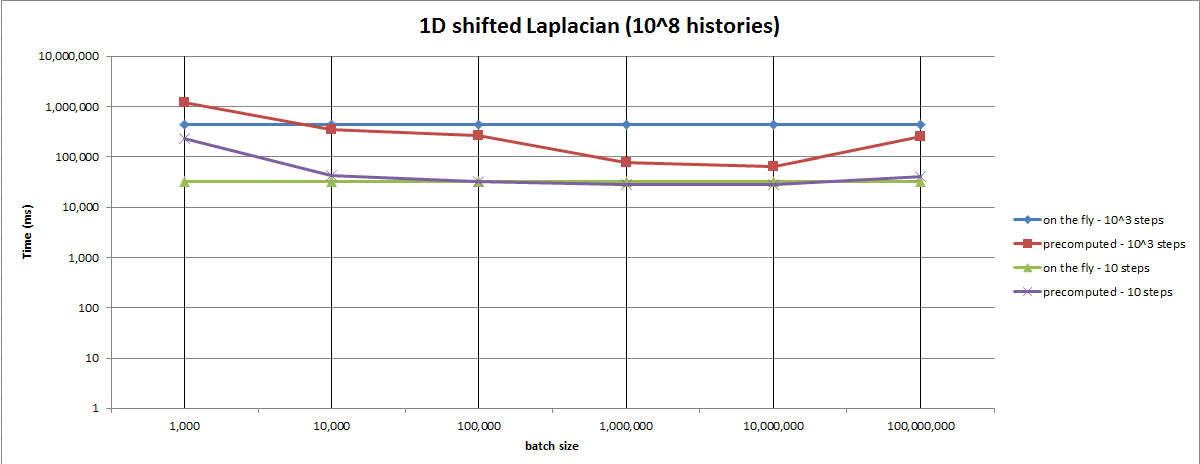
\includegraphics[width=\textwidth]{1d_lap_onthefly_vs_precompute.png}
    \caption{Adjoint method - OnTheFly vs. Precomputed approach. 1D shifted 
Laplacian.}
\label{1d_lap}
\end{figure}

\begin{figure}[h!]
  \centering
    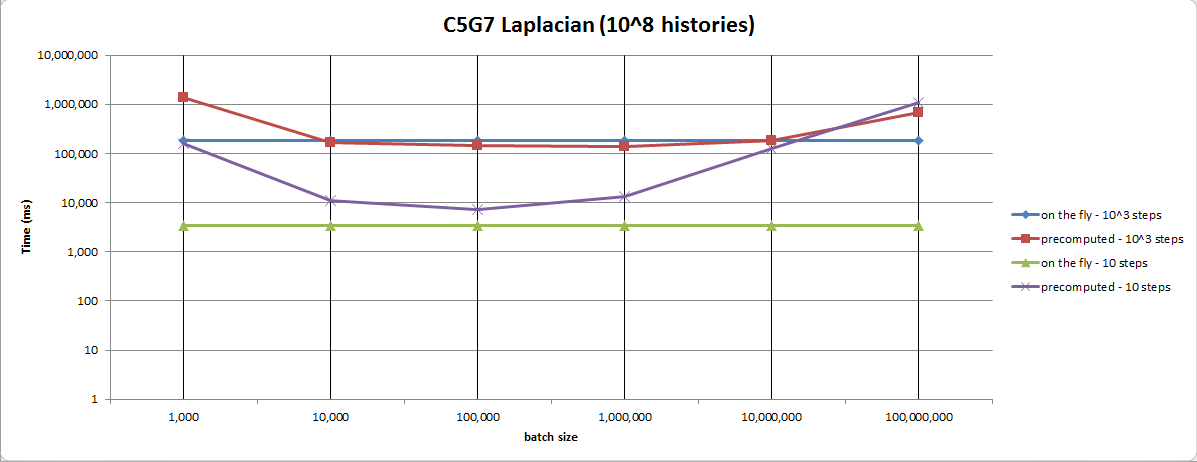
\includegraphics[width=\textwidth]{c5g7_onthefly_vs_precompute.png}
    \caption{Adjoint method - OnTheFly vs. Precomputed approach. $SP_1$ 
problem.}
\label{1d_lap}
\end{figure}

As you can notice, for the 1D shifted laplacian (Figure 
\textcolor{red}{figura}) a significant drop of the timing is achieved when the 
size of the batch assumes intermediate values with respect to the size of the 
problem ($10^6$). However, when these two values assume a comparable order of 
magnitude, a worsening of the performance is detected. Such behavior can be 
explained with the significant augmentation of atomic operation occurring. In 
fact the decrease of the batch size increases also the number of random walks 
starting from the same state, implying their request to modify the same value in 
the memory. 

As regards the $SP_1$ problem the situation is more problematic. In fact, 
regardless of the batch size, the Precomputed approach never succeeds in 
outperforming the standard way of proceeding. Moreover, an increase of the time 
along with the increase of the batch size is verified in this case as well. 
\newline

We employed the \texttt{NVIDIA} profiler to validate the theory that attributes 
the increase of the time to the enhancement of atomic operations.
A standard employment of such tool already provided us with useful information 
regarding the portion of the algorithm employing most of the time. In 
particular the 99\% of the time is spent to execute the 
\texttt{run\_adjoint\_monte\_carlo} kernel. This is a positive feedback, since 
it shows that almost the entire runtime is spent for the actual 
computation rather than for preprocessing or postprocessing operations.

Once this verified, a more detailed analysis of the performance is required to 
reach the goal of the validation. In particular, since we want to focus on 
profiling just the \texttt{run\_adjoint\_monte\_carlo} kernel, we can employ 
some \texttt{CUDA} subroutine to restrict the area profiled. 

To limit profiling to a region of your application, CUDA provides functions to 
start and stop profile data collection. \texttt{cudaProfilerStart()} is used to 
start profiling and \texttt{cudaProfilerStop()} is used to stop profiling. In 
order to make such calls effective, it is necessary to employ the metric 
\texttt{--profile-from-start off} when the command line profiler 
\texttt{nvprof} is called. If instead the visual profiler \texttt{nvvp} is 
employed, the previous calls must be combined by disabling the profiling from 
the start during the creation of the new session. \newline

The previous subroutines have been combined with the use of the compiling flag 
\texttt{-lineinfo} to generate line number information for applications 
without affecting the optimization level of the output. Differently from the 
standard debugging flag \texttt{-G}, \texttt{-lineinfo} does not force the 
compiler to generate debug information for the CUDA application. 


\end{document}
